\section{Geradlinige Dreiecks Darstellungen (SLTRs)}

Ausgehend von der konvexen Darstellung nach Tutte, kann man sich die Frage stellen unter welchen Vorraussetzungen wir einen planaren Graphen so zeichnen können, dass alle Gebiete, inklusive dem Äusseren Dreiecken umranden. Bei der Formalisierung dieser Darstellung und ersten Feststellungen halten wir uns an Nieke Aerts und Stefan Felsner \cite{af13}.

\begin{definition}[SLTR]\label{defsltr}
Eine Zeichnung eines planen Graphen $G$ wird Gradlinige Dreiecks Darstellung, im weiteren kurz \textit{SLTR} (für die englische Bezeichnung Staight Line Triangle Representation), genannt falls gilt:
\begin{itemize}
\item[S1] Alle Kanten Segmente von Geraden
\item[S2] Alle Gebiete, inklusive dem äusseren, sind nicht degenerierte Dreiecke.
\end{itemize}
\end{definition}

\begin{figure}[h]
	\centering
  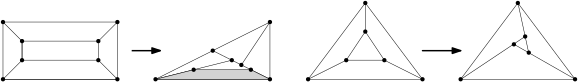
\includegraphics[width=0.9\textwidth]{sltr-example.png}
	\caption{Links einer der beiden drei-zusammenhängenden Graphen auf acht Knoten ohne SLTR und rechts ein Graph mit einer möglichen SLTR.}
\end{figure}

Um die Problemstellung greifbarer zu machen werden wir planare Graphen zusammen mit den drei Aufhängungen $a_1,a_2$ und $a_3$ als designierten Ecken einer möglichen SLTR betrachten. Einen Graphen zusammen mit einem äusseren Gebiet bzw. Aufhängungen zu betrachten, macht auch in sofern Sinn, dass kombinatorische Graphen existieren, von denen manche Einbettungen SLTRs zulassen, andere jedoch nicht, so wie in Abbildung \ref{10_example} zu sehen.

\begin{figure}
	\centering
  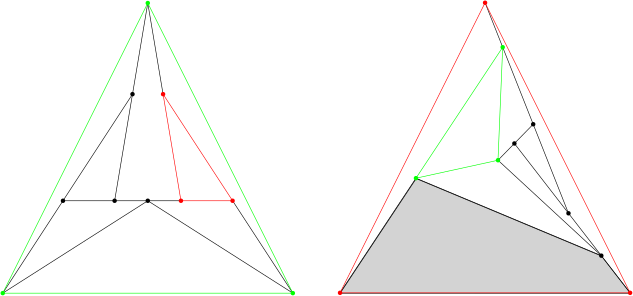
\includegraphics[scale=0.1]{10_example.png}
  	\label{10_example}
	\caption{Der kleinste drei-zusammenhängende kombinatorische Graph mit einer Wahl der Aufhängungen die eine SLTR zulässt und einer Auswahl ohne SLTR.}
\end{figure}

\begin{proposition}
Sei $G$ ein Graph mit Aufhängungen $a_1,a_2,a_3$ als äusseren Ecken einer SLTR. Weiter gebe es keinen Knoten von Grad zwei der in beiden angrenzenden Gebieten den Winkel $\pi$ hat\footnote{Ein solcher Knoten ist keine Aufhängung, da der Aussenwinkel grösser als $\pi$ ist. Alle anderen Knoten haben $\leq\pi$ Winkel. Somit können wir ihn durch eine gerade Kante zwischen seinen Nachbarn ersetzen und den resultierenden Graphen betrachten.}. Dann ist $G$ intern-drei-zusammenhängend\ref{int_3_con}.
\end{proposition}

%% TODO do i want the Proof??

Wir werden also von nun an, der Einfachheit halber intern-drei-zusammenhängende Graphen mit Aufhängungen betrachten, da alle anderen Graphen mit SLTR auf diese reduziert werden können. \\

Zu den Fragen, welche notwendigen und hinreichenden Bedingungen es für die Existenz von SLTRs gibt und  welche algorithmischen Ansätze es bei der Suche nach einer spezifischen Darstellung gibt haben Aerts und Felsner in \cite{af13}, \cite{af13h} und \cite{af15} schon einige Antworten geliefert, mit denen wir uns in den nächsten beidem Kapiteln beschäftigen werden. Zuerst müssen aber in diesem Kapitel noch ein paar notwendige Konzepte eingeführt werden.
